\documentclass[titlepage]{article}

\usepackage{fancyhdr}
\usepackage{layout}
\usepackage{titlesec}
\usepackage{indentfirst}

\usepackage{hyperref} 
\usepackage{graphicx}
\usepackage{amsmath}
\usepackage{amssymb}
\graphicspath{ {./images/} }

% Číslování
\pagenumbering{arabic}

\renewcommand{\contentsname}{Obsah}
\renewcommand{\refname}{Reference}

% ZDE ÚPRAVY ŠABLONY
\newcommand{\uloha}{Barevná čára/Coloured Line}
\newcommand{\datum}{22.12.2022}

% Titulní strana
\title{\uloha}
\author{Tým GCh(D+1)}
\date{\datum}

\begin{document}

% Horizontální margin
\hoffset=-0.5in
\textwidth=417pt
\linewidth=\textwidth
\hsize=\textwidth

% Vertikální margin
\voffset=-0.5in
\textheight=602pt

% Titulní strana
\begin{titlepage}
    \begin{center}

        \huge
        Turnaj mladých fyziků, 36. ročník(2022/2023)

        \vspace{1.5in}
        \LARGE
        \textbf{\uloha}

        \vspace{3in}
        \LARGE
        Gymnázium Christiana Dopplera, Gymnázium Cheb
        \linebreak
        Tým GCh(D+1)

        \vspace{1.7in}
        \large
        \datum

    \end{center}
\end{titlepage}

% Headery
\pagestyle{fancy}
\fancyhead{}
\fancyhead[C]{\uloha}

\tableofcontents

\pagebreak

% TO ASK:
% Move image sources to references, how to reference images???
% unifikovat vzdálenost, tloušťka

% Formát odstavců
\parindent=.25in
\parskip=.1in
\titlespacing*{\section}{0ex}{0ex}{0ex}
\titlespacing*{\subsection}{0ex}{0ex}{0ex}

\section{Zadání}

\subsection{Originální znění v angličtině}

When a compact disc or DVD is illuminated with light coming from a filament lamp in such a way that only rays with large angles of incidence are selected, a clear green line can be observed. The colour varies upon slightly changing the angle of the disc. Explain and investigate this phenomenon.

\subsection{Překlad zadání do češtiny}

Když osvítíme kompaktní disk nebo DVD světlem z žárovky s wolframovým vláknem tak, že jsou vybrány pouze paprsky s velkým úhlem dopadu, můžeme pozorovat jasnou zelenou čáru. Její barva se mění s nepatrnými změnami úhlu náklonu disku. Vysvětlete a prozkoumejte tento jev.

\section{Úvod}

\phantomsection \label{image:1}
\includegraphics[width=\textwidth]{illustration1.png}
\begin{center}
    Obrázek 1: Ilustrační obrázek ukazující barevné jevy při posvícení na kompaktní disk. \cite{img1}
\end{center}

\phantomsection \label{image:2}
\includegraphics[width=\textwidth]{illustration2.png}
\begin{center}
    Obrázek 2: Ilustrační obrázek ukazující obdobné barevné jevy při posvícení na DVD. \cite{img2}
\end{center}

Duhové jevy objevující se na DVD a kompaktních discích jsou charakteristickou a jednoduše pozorovatelnou vlastností těchto často používaných datových médií.

V našem řešení identifikujeme hlavní fenomény vedoucí k těmto jevům a jejich zbarvení. Vytvoříme a experimentálně potvrdíme modely pro nejdůležitější fenomény a zmíníme další druhotné fenomény.

\pagebreak

\section{Ustanovení terminologie}
V níže uvedené tabulce 1 definujeme značení parametrů používaných v celém dokumentu.

\begin{center}
    \phantomsection \label{table:1}
    Tabulka 1: Stanovené značení používaných parametrů s vysvětlením. \\[3px]
    \begin{tabular}{c c c}
        Typ parametru & Značka   & Význam                                                                                       \\[1px]
        \hline
        bod           & $S$      & Střed disku                                                                                  \\
        bod           & $L$      & Bodový zdroj světla                                                                          \\
        bod           & $O$      & Pozorovatel                                                                                  \\
        bod           & $P$      & Pozorovaný bod                                                                               \\
        bod           & $A$      & Bod na obvodu disku umístěný kolmo pod úsečkou $LS$                                          \\
        bod           & $B$      & Bod na obvodu disku umístěný kolmo pod polopřímkou $\overset{\longmapsto}{LS} $ ($A \neq B$) \\
        vzdálenost    & $p$      & Tzv. \emph{pitch*} disku                                                                     \\
        vzdálenost    & $h$      & Tloušťka polykarbonátové (PC) vrstvy disku                                                   \\
        úhel          & $\alpha$ & $\angle LPA$                                                                                 \\
        úhel          & $\beta$  & $\angle OPB$                                                                                 \\
        \hline
    \end{tabular}
\end{center}
Poznámky: \\
\emph{* pitch} = standardizovaná vzdálenost datových drah na optických discích

\section{Teorie}

\subsection{Fenomenologický popis}
Předtím, než začneme, je nutné zmínit následující předpoklady pro následující modely:
\begin{enumerate}
    \item \phantomsection \label{approx:1} Zdroj světla aproximujeme jako bodový zdroj světla chovající se jako absolutně černé těleso.
    \item \phantomsection \label{approx:2} Pro makroskopické účely zdroj světla vyzařuje radiálně do všech směrů z bodu $L$.
    \item \phantomsection \label{approx:3} Pro makroskopické účely zanedbáme tloušťku $h$ disku samotného, protože $|LP| >> h$.
    \item \phantomsection \label{approx:4} Pro mikroskopické účely aproximujeme směr blízkých paprsků světla na paprsky rovnoběžné (quasiparalelní), protože $|LP| >> p$.
\end{enumerate}

\pagebreak

Světlo vycházející ze zdroje s diskem interaguje na dvou místech - při vstupu do PC vrstvy a při odrazu od hliníkové vrstvy s datovou stopou. Toto povede ke dvěma hlavním fenoménům, jmenovitě lomu a difrakci.

\subsection{Difrakce a stavba optických disků}
\begin{center}
    \phantomsection \label{image:3}
    \includegraphics[width=8cm]{construction1.png}
    \linebreak
    Obrázek 3: Diagram znázorňující průřez (ne v měřítku) optickým médiem společně s využitím destruktivní interference pro čtení datové dráhy.  \cite{img3}
\end{center}

K difrakci na hliníkové vrstvě optických disků může docházet díky měnící se topologii vrstvy. Datová stopa je totiž složena z \emph{pitů} a \emph{landů}.
Pit je oblast se vzdáleností od čtecího povrchu disku o $\lambda/4$ větší nežli land, kde $\lambda$ reprezentuje vlnovou délku čtecího laseru v polykarbonátovém prostředí.
Při přechodu z pitu na land tedy dochází k rozdílu uražené dráhy dvou blízkých rovnoběžnách paprsků o $\lambda/2$, což způsobuje destruktivní interferenci (viz \hyperref[image:3]{obrázek 3}).Tato destruktivní interference je poté zaznamenána jako binární hodnota 1 \cite{optical_disc}.
% ZdrojX: http://www.laesieworks.com/digicom/Storage_CD.html
% ZdrojX: https://slideplayer.com/slide/7228632/
% ZdrojX: https://slideplayer.com/slide/14796174/

\pagebreak

\phantomsection \label{image:4}
\includegraphics[width=\textwidth]{construction2.png}
\begin{center}
    Obrázek 4: Diagram znázorňující rozdílnou stavbu jednotlivých datových médií.\cite{img4}
\end{center}

Podobnost vlnové délky viditelného světla (cca 380nm - 750nm) a pitche CD (cca 1600 nm) nebo DVD (cca 740 nm) společně s již zmíněnou topologií hliníkové vrstvy způsobuje další difrakční jevy podle Huygens-Fresnelova principu.
Díky častému opakování těchto difrakčních ploch se celek hliníkové vrstvy chová také jako difrakční mřížka.

\subsection{Lom}
Světlo přicházející do PC vrstvy disku může vcházet čtecí stranou disku, kdy prochází celou tloušťkou této PC vrstvy, nebo může také vstoupit obvodovou stranou disku, která je 1.2mm vysoká (viz \hyperref[image:4]{obrázek 4}).
Ty se na přechodu prostředí budou lámat podle Snellova zákona, kde index lomu polykarbonátu $n_{PC} \approx 1.585$ \cite{index_lomu}.
% ZdrojX: https://refractiveindex.info/?shelf=organic&book=polycarbonate&page=Sultanova

\pagebreak

\phantomsection \label{subsubsec:4.3.1}
\subsubsection{Lom horní plochou}

\phantomsection \label{image:5}
\includegraphics[width=\textwidth]{microdrawing.png}
\begin{center}
    Obrázek 5: Nákres mikroskopického náhledu na lom světla na rozhraní optických prostředí polykarbonátu a okolí. (ne v měřítku)
\end{center}

Uvážíme-li dva blízké paprsky $a$ a $b$ dopadající na horní (čtecí) plochu splňující \hyperref[approx:4]{předpoklad 4}, které po průchodu PC vrstvou dopadají na landy (viz \hyperref[image:5]{obrázek 5}) a přicházejí z bodového zdroje světla ve fázi, bude u nich docházet k předbíhání jednoho paprsku před druhým, protože netráví ve stejných prostředích stejný čas.
Bez újmy na obecnosti můžeme říci, že paprsek $a$ dopadá na disk dále od zdroje světla.
V tomto případě is dráhu, o kterou se paprsek opozdí při vstupu do prostředí, označíme $\Delta s_a$ a analogický jev při výstupu paprsku $b$ označíme $\Delta s_b$.
Celkový rozdíl uražených drah je tedy:
\begin{equation}
    \label{eq1}
    \Delta s = \Delta s_a - \Delta s_b = p \cdot (\cos{\alpha} - \cos{\beta})
\end{equation}

Všimněme si, že úhel $\beta$ může nabývat i hodnot $>90$° a i tyto hodnoty nás zajímají (na rozdíl od úhlu $\alpha$, kde nás zajímají hlavně malé velikosti tohoto úhlu). V případě, že by úhel $\beta$ nabyl hodnot $>90$°, bude $\Delta s_b$ nabývat hodnot záporných, což je ekvivalentní tomu, kdyby $\Delta s_a$ bylo o $|\Delta s_b|$ zvětšeno, k čemuž podle našeho modelu má dojít. Díky tomuto je tento model stále logický.

\subsubsection{Hypotéza 1}
\phantomsection \label{hyp:1}
Naše hypotéza využívá konstruktivní interference a vychází z \hyperref[eq1]{rovnice 1}.
Dle naší hypotézy dochází ke konstruktivní interferenci specifické vlnové délky světla $\lambda$, pokud se opoždění paprsků bude rovnat $k$-násobku $\lambda$.
Jsme tedy schopni postavit rovnici, ze které v závislosti na konfiguraci parametrů můžeme určit konstruktivně interferovanou vlnovou délku světla.
Rovnice zní:

\begin{equation}
    \label{eq2}
    k\lambda = p \cdot (\cos{\alpha} - \cos{\beta}) \ \ \ \ \ \  k \in \mathbb{N}
\end{equation}

\begin{equation}
    \label{eq3}
    \lambda = \frac{ p \cdot (\cos{\alpha} - \cos{\beta}) }{k}
\end{equation}

Pokud empirické měření bude splňovat tuto podmínku, potvrdíme tím tuto hypotézu (viz \hyperref[exp:1]{sekce 5.1}).
Zároveň také tento jev bude způsobovat destruktivní interferenci pro hodnoty $k = n + \frac{1}{2}$, kde $n \in \mathbb{N}$.

\subsubsection{Lom obvodovou stranou}

\phantomsection \label{image:6}
\includegraphics[width=\textwidth]{repeatedrefelction.png}
\begin{center}
    Obrázek 6: Nákres lomu světla vstupujícího na obvodové straně.
\end{center}

Uvážíme-li jiný případ, kdy máme paprsek dopadající na obvodovou stranu pod malým úhlem $\alpha$, bude uvnitř polykarbonátové vrstvy docházet k opakovanému odrazu, kde při každém odrazu dojde podle Fresnelových vztahů k vyzáření části energie z PC vrstvy ven.

\subsubsection{Hypotéza 2}
\phantomsection \label{hyp:2}

Druhá hypotéza zní následovně - Protože uvnitř polykarbonátové vrstvy dochází k opakovanému odrazu, kde při každém odrazu dojde podle Fresnelových vztahů k vyzáření části energie ven, po použití Snellova zákona jsme tedy schopni vypočítat vzdálenost jednotlivých míst vyzáření $l$ v závislosti na úhlu $\alpha$ takto:

\begin{equation}\label{eq4}
    \begin{gathered}
        \frac{\sin(\alpha')}{\sin(\alpha)} = \frac{n_0}{n_{PC}} \\
        \alpha' = \arcsin{\left(\sin(\alpha) \cdot \frac{n_0}{n_{PC}}\right)}
    \end{gathered}
\end{equation}

\begin{equation}\label{eq5}
    \begin{gathered}
        \alpha' = \frac{2h}{l}
    \end{gathered}
\end{equation}

\begin{equation}\label{eq6}
    \begin{gathered}
        \arcsin{\left(\sin(\alpha) \cdot \frac{n_0}{n_{PC}}\right)} = \frac{2h}{l} \\
        l = \frac{2h}{\tan{\left(\arcsin{\left(\sin(\alpha) \cdot \frac{n_0}{n_{PC}}\right)}\right)}}
    \end{gathered}
\end{equation}

\hyperref[eq4]{Rovnice 4} využívá Snellova zákona.
\hyperref[eq5]{Rovnice 5} vychází z geometrického nákresu na \hyperref[image:6]{obrázku 6}.
Pokud empirické měření bude splňovat tuto podmínku, potvrdíme tím tuto hypotézu (viz \hyperref[exp:2]{sekce 5.2}).

\section{Praxe}

\phantomsection
\label{exp:1}
\subsection{Experiment 1 - konstruktivní interference při vstupu světla horní plochou}

V prvním experimentu se budeme snažit sledovat a dokázat konstruktivní interferenci zmiňovanou v \hyperref[hyp:1]{hypotéze 1} pomocí fotografického záznamu.

\subsubsection{Aparatura a pomůcky}

Mezi použité pomůcky patří:
\begin{enumerate}
    \item DVD-R a CD-R disky
    \item Digitální fotoaparát s dlouhou expozicí pro zachycení barev na disku
    \item Zdroj světla ve formě lampy s wolframovým vláknem
    \item Posuvné měřítko pro určení rozměrů disků a relativních pozic objektů (rozlišení 0.1mm)
\end{enumerate}

Nákresy aparatury dle \hyperref[table:1]{stanoveného značení}:

\phantomsection \label{image:7}
\begin{center}
    \includegraphics[width = \textwidth]{exp1_d1.png}
    \linebreak
    Obrázek 7: Nákres aparatury pro experiment 1 z profilu.
\end{center}

\phantomsection \label{image:8}
\begin{center}
    \includegraphics[width = \textwidth]{exp1_d2.png}
    \linebreak
    Obrázek 8: Nákres aparatury pro experiment 1 shora.
\end{center}

\subsubsection{Provedení}

Nejprve byly objekty rozmístěny a byl vybrán bod $P = A$ (pro jednoduchost).
Byl použit DVD disk.
Vzdálenosti jednotlivých objektů v  měřící rovině byly následující:

\begin{equation}\label{eq7}
    \begin{gathered}
        l_x = P_x - L_x = 70cm \\
        l_y = P_y - L_y = 3cm \\
        c_x = P_x - O_x = 77.5cm \\
        c_x = P_y - O_y = -35cm \\
    \end{gathered}
\end{equation}

V místosti byla zhasnuta všechna světla kromě nášeho zdroje světla s wolframovým vláknem a fotoaparát byl nastaven na dlouhou expozici, aby byl schopen vytvořit kvalitní fotografii, i přestože je v místosti značné šero.

Ze vzdáleností $l_x, l_y, c_x$ a $c_y$ dopočítáme úhly $\alpha$ a $\beta$.

\begin{equation}\label{eq8}
    \begin{gathered}
        \alpha = atan \left(\frac{l_y}{l_x}\right) \\
        \alpha = 2.45^{\circ} \\ \\
        \beta = atan \left(\frac{c_y}{c_x}\right) \\
        \beta = 114.305^{\circ} \\
    \end{gathered}
\end{equation}

Finálně aplikujeme náš model z \hyperref[hyp:1]{hypotézy 1} podle konstrukce DVD z \hyperref[image:4]{obrázku 4}.

\begin{equation}\label{eq9}
    \begin{gathered}
        k\lambda = p \cdot (\cos{\alpha} - \cos{\beta}) \\
        k\lambda = 740 nm \cdot (\cos{2.45^{\circ}} - \cos{114.305^{\circ}}) \\
        k\lambda = 1043.9 nm \\ \\
        \textnormal{pro } k = 2 \\
        \lambda = 521.95 nm
    \end{gathered}
\end{equation}

Dle modelu očekáváme tedy světlo s vlnovou délkou kolem 521.95 nm.

\subsubsection{Výsledky}

Barva našeho bodu $P$ by tedy měla být zelená, jelikož vlnová délka zelené barvy se pohybuje v rozhraní cca 495–570 nm. Toto se potvrzuje i z fotografie pořízené při měření níže (viz \hyperref[image:8]{obrázek 8}):

\phantomsection \label{image:8}
\begin{center}
    \includegraphics[height=7.5cm]{exp1_v.png}
    \linebreak
    Obrázek 8: Fotografie z experimentu 1 s DVD s popisky.
\end{center}

Další obdobné experimenty s kompaktním diskem byly provedeny a jejich výsledky jsou uvedeny níže (viz \hyperref[table:2]{tabulka 2}, \hyperref[image:9]{obrázky 9} a \hyperref[image:10]{10}) (pro každý platí, že $l_y = 23.2mm$ a $c_y = 143.2mm$):

\label{table:2}
\begin{center}
    Tabulka 2: Tabulka měření experimentu 1 pro CD. \\[3px]
    \begin{tabular}{ c | c | c  | c || c | c | c || c | c }
        Bod   & $l_x$ [mm] & $c_x$ [mm] & $k$ & $\alpha$ & $\beta$ & $\lambda$ [nm] & Teoretická barva & Sledovaná barva \\
        \hline
        $P_1$ & 127.63     & 30         & 2   & 10.3°    & 78.2°   & 623            & Oranžová         & Světle oranžová \\
        $P_2$ & 147.63     & 10         & 3   & 8.93°    & 86.0°   & 490            & Tyrkysová        & Tyrkysová       \\
        $P_3$ & 167.63     & -10        & 3   & 7.88°    & 94.0°   & 565            & Zelená           & Zelená          \\
        $P_4$ & 247.25     & 30         & 2   & 5.36°    & 78.2°   & 632            & Oranžová         & Oranžová        \\
        $P_5$ & 167.25     & 10         & 3   & 4.96°    & 86.0°   & 494            & Tyrkysová        & Tyrkysová       \\
        $P_6$ & 187.25     & -10        & 3   & 4.62°    & 94.0°   & 569            & Žluto-zelená     & Zelená          \\
        \hline
    \end{tabular}
\end{center}


Fotografie z experimentu 1 pro CD:

\phantomsection \label{image:9}
\phantomsection \label{image:10}
\begin{center}
    \includegraphics[height=7cm]{exp1_v_close.png}
    \includegraphics[height=7cm]{exp1_v_far.png}
    \linebreak
    Obrázky 9 a 10: Fotografie z experimentu 1 s CD s popisky.
\end{center}

Jak je z měření zřejmé, tyto barevné artefakty opravdu odpovídají teoretickému modelu z \hyperref[hyp:1]{hypotézy 1}. Kvalitnějších výsledků jsme dosáhli při větší vzdálenosti zdroje světla od disku, ale měření z větší blízkosti dosahuje poměrně uspokojivých výsledků.

Pro situace, kdy máme malý úhel $\alpha$ a velkou vzdálenost pozorovatele od disku se může tedy podle našeho modelu celá čára jevit zelená, jelikož rozdílná pozice bodu $P$ nebo bodu $O$ má pouze malý efekt na úhel $\beta$. Přiblížením bodu $O$ k disku se začnou objevovat i další barvy.

\phantomsection
\label{exp:2}
\subsection{Experiment 2 - vnitřní odraz při vstupu světla obvodovou stranou}

V druhém experimentu se budeme snažit sledovat opakující se odrazy v PC vrstvě DVD disku podle modelu z \hyperref[hyp:1]{hypotézy 2}. Jelikož se nejedná o interferenční jev, použijeme libovolný zdroj světla.

\subsubsection{Aparatura a pomůcky}

Mezi použité pomůcky patří:
\begin{enumerate}
    \item DVD-R disk
    \item Fotoaparát mobilního telefonu
    \item Zdroj světla ve formě svítilny mobilního fotoaparátu
    \item Posuvné měřítko pro určení rozměrů disků a relativních pozic objektů (rozlišení 0.1mm)
    \item Clonu ve formě plastové kostky pro odstínění okolního světla
    \item Tmavá látka pro podložení disku
\end{enumerate}

Nákresy aparatury dle \hyperref[table:1]{stanoveného značení}:

\phantomsection \label{image:11}
\begin{center}
    \includegraphics[width=\textwidth]{exp2_d1.png}
    \linebreak
    Obrázek 11: Nákres aparatury pro experiment 2 z profilu.
\end{center}

\phantomsection \label{image:12}
\begin{center}
    \includegraphics[width=\textwidth]{exp2_d2.png}
    \linebreak
    Obrázek 12: Nákres aparatury pro experiment 2 shora.
\end{center}

\subsubsection{Provedení}

Disk byl položen na tmavou látku a byla připravena clona, která bude co nejlépe bránit radiálním paprskům svítilny mobilního telefonu v zasahování horní plochy DVD disku, aby byla zlepšena viditelnost jevu.
Do vyměřené pozice byla umístněna svítilna a pomocí posuvného měřítka byla vyměřena průměrná vzdálenost míst vyzáření z PC.
Jev může být pozorovám z libovolné pozice bodu $O$.
Jev byl sledován ve dvou různých konfiguracích.

\subsubsection{Výsledky}

V níže uvedené \hyperref[table:3]{tabulce} jsou určeny parametry systému a porovnání teoretické a měřené hodnoty $l$ použitím vzorce z \hyperref[eq6]{rovnice 6} pro $n_{PC} = 1.585$ \cite{index_lomu} a $n_0 = 1$ (přibližná hodnota pro vzduch):

\label{table:3}
\begin{center}
    Tabulka 3: Tabulka měření experimentu 2 společně s odchylkou. \\[3px]
    \begin{tabular}{ c | c | c || c || c | c | c }
          & $l_x$ [cm] & $l_y$ [cm] & $\alpha$ & Teoretické $l$ [mm] & Měřené $l$ [mm] & $\delta$ \\
        \hline
        1 & 18         & 6.5        & 19.86°   & 5.47                & 5.3             & 4.58\%   \\
        2 & 14.2       & 12.5       & 41.36°   & 2.62                & 2.67            & 1.87\%   \\
        \hline
    \end{tabular}
\end{center}

A fotografie z experimentu 2:

\phantomsection \label{image:13}
\phantomsection \label{image:14}
\begin{center}
    \includegraphics[width = 6.5cm]{exp2_1.png}
    \includegraphics[width = 6.5cm]{exp2_2.png}
    \linebreak
    Obrázky 13 a 14: Fotografie z experimentu 2. Měření 1 vlevo, měření 2 vpravo.
\end{center}

Jasné opakující se bílé čáry potvrzují \hyperref[hyp:2]{hypotézu 2}. Dále se dá také sledovat, že oddálením zdroje světla dojde k zostření bílých čar, což dle našeho modelu vychází z toho, že paprsky světla budou quasiparalelnější, pokud budou přicházet z větší vzdálenosti.

Jednou z příčin odchylek mohla být například nerovnost boční strany DVD disku, která mohla zapřičiňovat rozdílnost úhlu $\alpha$, protože při měření se předpokládalo, že boční strana bude kolmá na rovinu podložky, což nemusí být pravda.

\phantomsection \label{sec:other_fen}
\section{Další pozorované fenomény}

Jedním z dalších pozorovaných fenoménů je změna úhlu mezi barvenou čárou, která se objevuje díky \hyperref[hyp:1]{hypotéze 1}, a úsečkou $AB$.
V \hyperref[exp:1]{experimentu 1} je celá měřící aparatura vložena do jedné roviny, čímž byl problém redukován do 2D.
Pokud ale bod $O$ vyjmeme z této roviny, dojde ke změně úhlu $\angle ASP$.

Dle naší hypotézy bude k tomuto jevu docházet díky tomu, že jednotlivé datové trasy budou mít přibližný tvar koncentrických polotorů.
Doopravdy se bude jednat o jednu dlouhou zaoblenou spirálu, ale v malé oblasti toto dělá zanedbatelný rozdíl.

Na povrchu těchto drah dochází k odrazu světla a následně také ke konstruktivní interferenci, jak bylo popsáno v \hyperref[subsubsec:4.3.1]{sekci 4.3.1}. Světlo putující v rovině $LSO$ se může odrážet od jednotlivých torů. Označíme-li si bod odrazu viděného paprsku jako $U$ a střed úsečky $LO$ jako $X$ (který leží na ose úhlu $\angle LSO$, což je zřejmé), musí platit, že úhel dopadu a úhel odrazu bude stejný.
Budeme-li počítat všechny paprsky jako quasiparalelní, protože $|LS| >> p$, můžeme říci, že bod $U$ bude ležet na průniku osy úhlu $\angle LSO$ a daného toru.
Pokud tuto proceduru zopakujeme pro každý torus, budou všechny body odrazu ležet na jedné přímce, která odpovídá průnětu osy úhlu $\angle LSO$ do podložky. Přibližný 3D nákres na následujících \hyperref[image:15]{obrázcích 15} a \hyperref[image:16]{16}:

\phantomsection \label{image:15}
\begin{center}
    \includegraphics[width = 11cm]{3D_1.png}
    \linebreak
    Obrázek 15: Detailní náhled na 3D aproximaci interakcí paprsků v tory.
\end{center}

\phantomsection \label{image:16}
\begin{center}
    \includegraphics[width = 11cm]{3D_2.png}
    \linebreak
    Obrázek 16: Vzdálený náhled na 3D aproximaci interakcí paprsků s tory.
\end{center}

\pagebreak

Body $U_{1}$ a $U_{2}$ jsou body, ve kterých se paprsky putující touto rovinou odrážejí. Je vidět, že $\angle OU_1X \approx \angle LU_1X$ a $\angle OU_2X \approx \angle LU_2X$. To, že nejsou přesně rovny vychází z toho, že v přibližném 3D modelu se body $O$ a $L$ nachází značně blíže, než v realitě. 
Toto je provedeno čistě za účelem zpraktičnění a zjednodušení tvorby 3D modelu.

V modelu je menší poloměr $r$ torů roven jedné arbitrární jednotce a body $O$ a $L$ jsou ve vzdálenosti cca 40 arbitrárních jednotek od středu $S$.
Pokud bychom chtěli v modelu reprezentovat pozice podle reálného měřítka, museli bychom bod $L$, který by byl ve vzdálenosti např. 70cm od středu $S$, umístit do vzdálenosti 
$\frac{70cm}{160nm}=4375000 \textnormal{ arbitrárních jednotek}$ pro DVD a $\frac{70cm}{300nm} = 2333333 \textnormal{ arbitrárních jednotek}$ pro CD v modelu, což jsme se rozhodli čistě z nepraktičnosti věci nedělat.
Pokud bychom toto uděli, vedlo by to na ještě lepší výsledky, protože bychom zvýšili quasiparalelnost paprsků.
Body $U_1$ a $U_2$ jsou poté zobrazeny na body $V_1$ a $V_2$ kolmo do roviny podložky.

\phantomsection \label{image:17}
\begin{center}
    \includegraphics[width = 8cm]{other_fen_1.png}
    \linebreak
    Obrázek 17: Fotografie disku kolmo shora se zdrojem světla ve velké vzdálenosti (po pravé straně). Body $S, L$ a $O$ tvoří rovinu kolmou k podložce jako v \hyperref[exp:1]{experimentu 1}. Bílé značky označují velikosti úhlů 0°, 45° a 90° vůči $AB$.
\end{center}

\phantomsection \label{image:18}
\begin{center}
    \includegraphics[width = 10cm]{other_fen_2.png}
    \linebreak
    Obrázek 18: Fotografie disku z boku se zdrojem světla ve velké vzdálenosti a s bodem $O$ pod malým úhlem ve střední vzdálenosti. Body $S, L$ a $O$ tvoří rovinu nekolmou k podložce. Čára vyznačena červeně. Úhel 45° stupňů vyznačen modře.
\end{center}

\phantomsection \label{image:19}
\begin{center}
    \includegraphics[width = 10cm]{other_fen_3.png}
    \linebreak
    Obrázek 19: Fotografie disku z boku se zdrojem světla ve velké vzdálenosti a s bodem $O$ pod velmi malým úhlem ve velké vzdálenosti (fotografie přiblížena). Čára vyznačena červeně. Úhel 45° stupňů vyznačen modře.
\end{center}

Jak vidíme na \hyperref[image:17]{obrázku 17}, čára je viditelná jak bychom předpokládali, když jsou body $S, L, O$ v rovině kolmé na podložku, stejně jako v \hyperref[exp:1]{experimentu 1}.
Při naklonění do strany, tedy změnšení úhlu mezi rovinou podložky a přímkou $\overset{\longleftrightarrow}{OS}$, dochází k odklonění čáry (viz \hyperref[image:18]{obrázek 18}), jak bychom předpokládali a při ještě menším úhlu se čára limitně blíží úhlu 45° (viz \hyperref[image:19]{obrázek 19}), protože úhel $\angle LSO$ je v tomto případě 90°. Toto odpovídá našemu geometrickému \hyperref[sec:other_fen]{modelu}.
(Poznámka: ostatní barevné artefakty vychází z okolního světla, které nebylo odstíněno a nejsou pro nás zajímavé.)

Čára se zároveň steným principem ukazuje i na opačné straně, bodově symetricky podle bodu S.

Z těchto poznatků a díky potvrzení naší hypotézy jsme tedy schopni utvořit geometrickou závislost úhlu $\angle LSP$ (dále $\gamma$) na úhlu $\angle LSO$ (dále $\theta$) a úhlu mezi podložkou a přímkou $\overset{\longleftrightarrow}{OS}$ (dále $\phi$):

\begin{equation}\label{eq9}
    \begin{gathered}
        \gamma = \frac{1}{2} \theta \cdot \cos{\phi}
    \end{gathered}
\end{equation}

Zároveň, pokud přiblížíme zdroj světla velmi blízko k disku, můžeme sledovat, že se čára začne zakřivovat (viz \hyperref[image:20]{obrázek 20} níže), protože začneme znatelně porušovat quasiparalelnost jednotlivých paprsků světla, což náš \hyperref[sec:other_fen]{model} vyžaduje.

\phantomsection \label{image:20}
\begin{center}
    \includegraphics[width = 10cm]{other_fen_4.png}
    \linebreak
    Obrázek 20: Fotografie disku ze strany se zdrojem světla velmi blízko. Čára vyznačena červeně.
\end{center}

\section{Závěr}

V průběhu této práce se nám povedlo vysvětlit původ barevných jevů, které vznikají na povrchů optických disků, jmenovitě CD a DVD disků. Zjistili jsme, že se jedná o více různorodých jevů založených hlavně na konstruktivní interferenci a opakovaném odrazu, kde každý z nich produkuje jinak vypadající světelný jev.

Podařilo se nám teoreticky modelovat 3 různé jevy, které jsme úspěšně experimentálně potvrdili za některých základních předpokladů. Podařilo se nám také sledovat jiné chování v případech, kdy tyto předpoklady nebyly dodrženy.

Možným budoucím rozšřením této práce by dle nás mělo být obecnější vysvětlení již zmíněných jevů, což by v důsledku dovolilo popsat větší množství jevů. Dále by také stály za zkoumání další, ještě námi nepopsané, jevy.

\pagebreak

\addcontentsline{toc}{section}{Reference}
\begin{thebibliography}{9}

    \bibitem{index_lomu}
    N. Sultanova, S. Kasarova and I. Nikolov. Dispersion properties of optical polymers, \href{http://przyrbwn.icm.edu.pl/APP/ABSTR/116/a116-4-42.html}{Acta Physica Polonica A 116, 585-587 (2009)} (fit of the experimental data with the Sellmeier dispersion formula: Mikhail Polyanskiy), zobrazeno 20.12.2022, \href{https://refractiveindex.info/?shelf=organic&book=polycarbonate&page=Sultanova}{https://refractiveindex.info/?shelf=organic\&book=polycarbonate\&page=Sultanova}

    \bibitem{optical_disc}
    Giesbert Nijhuis, zobrazeno 20.12.2022, \href{http://www.laesieworks.com/digicom/Storage_CD.html}{http://www.laesieworks.com/digicom/Storage\_CD.html}

    \bibitem{img1}
    Jon Abe, 10.9.2014, photo1.png, zobrazeno 20.12.2022, \href{https://joabe808.wordpress.com/2014/09/10/optics-cd-rainbow-reflection/}{https://joabe808.wordpress.com/2014/09/10/optics-cd-rainbow-reflection/}

    \bibitem{img2}
    Trisha, 25.4.2012, DVD-Rainbow.jpg, zobrazeno 20.12.2022, \href{https://inspirationlaboratories.com/how-to-make-a-rainbow/dvd-rainbow/}{https://inspirationlaboratories.com/how-to-make-a-rainbow/dvd-rainbow/}

    \bibitem{img3}
    \href{https://engineering.stackexchange.com/users/272/chris-mueller}{
        Chris Mueller
    }, 26.6.2015, wOhON.gif, zobrazeno 20.12.2022, \href{https://engineering.stackexchange.com/questions/3324/why-is-it-more-reliable-to-use-the-land-pit-transition-in-a-cd-rom}{https://engineering.stackexchange.com/questions/3324/why-is-it-more-reliable-to-use-the-land-pit-transition-in-a-cd-rom}

    \bibitem{img4}
    \href{https://commons.wikimedia.org/wiki/User:Cmglee}{Cmglee}, 6.6.2021, File:Comparison\_CD\_DVD\_HDDVD\_BD.svg,  zobrazeno 20.12.2022, \href{https://en.wikipedia.org/wiki/Comparison_of_high-definition_optical_disc_formats}{https://en.wikipedia.org/wiki/Comparison\_of\_high-definition\_optical\_disc\_formats}

\end{thebibliography}

\end{document}